% Created 2024-09-02 Mon 09:34
% Intended LaTeX compiler: pdflatex
\documentclass[aspectratio=169,xcolor={dvipsnames,svgnames}]{beamer}
\usepackage[utf8x]{inputenc}
\usepackage[T1]{fontenc}
\usepackage{graphicx}
\usepackage{longtable}
\usepackage{wrapfig}
\usepackage{rotating}
\usepackage[normalem]{ulem}
\usepackage{amsmath}
\usepackage{amssymb}
\usepackage{capt-of}
\usepackage{hyperref}
\usepackage{minted}
\usepackage{libertine}
\usepackage[normalem]{ulem}
\usepackage{varwidth}
\usepackage[Export]{adjustbox}
%\usepackage{enumitem}
\usepackage[linesnumbered,ruled,vlined]{algorithm2e}
\graphicspath{ {./careful-Isaac-Images/} {./org-download-images/} }
\usepackage[date=year,%
backend=biber,%
style=alphabetic,%
maxnames=5,%
minnames=3,%
maxalphanames=4,%
minalphanames=3,%
backref=true,%
doi=false,%
isbn=false,%
url=false,%
eprint=false]{biblatex}
\DefineBibliographyStrings{english}{%
backrefpage  = {\lowercase{s}ee p.}, % for single page number
backrefpages = {\lowercase{s}ee pp.} % for multiple page numbers
}
\addbibresource{/home/bvraghav/bibliography.bib}
%% Math typesetting
%% --------------------------------
\usepackage{amsmath}
\usepackage{amssymb}
\usepackage{amsfonts}
\usepackage{bbold}
% Operators with limit-style sub and superscript
\DeclareMathOperator*{\E}{\mathbb{E}}
\hypersetup{%
colorlinks=true,%
allcolors=magenta,%
%linkbordercolor = {white},%
%<your other options...>,
}
\usetheme{boxes}
\usecolortheme{crane}
\usefonttheme{serif}
\useinnertheme{rectangles}
\useoutertheme{}
\date{}
\title{mca101 : computer graphics}
\subtitle{2d geometry representation}
\author{%
%\noindent{} \\[2em]
\normalsize Raghav B. Venkataramaiyer
}
\institute{%
CSED TIET Patiala India.
}
\date{\scriptsize \today}
\setbeamercolor{alerted text}{fg=red!80!black}
%% Setup outline at begin section
%% -------------------------------------------------------
\AtBeginSection[]               % Section
{
\begin{frame}{outline}
\tableofcontents[currentsection,hideallsubsections]
\end{frame}
}
\AtBeginSubsection[]            % SubSection
{
\begin{frame}{outline}
\tableofcontents[currentsection,currentsubsection,subsectionstyle=show/shaded/hide]
\end{frame}
}
\setbeamerfont{structure}{shape=\scshape,family=\sffamily}
\setbeamertemplate{section page}
{
\begin{centering}
\begin{beamercolorbox}[sep=12pt,center]{part title}
\usebeamerfont{section title}\insertsection\par
\end{beamercolorbox}
\end{centering}
}

\setbeamercovered{transparent}
\hypersetup{
 pdfauthor={B.V. Raghav},
 pdftitle={mca101 : computer graphics},
 pdfkeywords={},
 pdfsubject={},
 pdfcreator={Emacs 29.4 (Org mode 9.6.24)}, 
 pdflang={English}}
\begin{document}

\maketitle

\section{2d geometry --- introduction}
\label{sec:org031ee22}

\subsection{Straight Lines}
\label{sec:orgf44613e}

\begin{frame}[label={sec:org512e054}]{\(y = mx + c\)}
\begin{align}
  \notag
  y = f(x) &= mx + c
\end{align}

\begin{center}
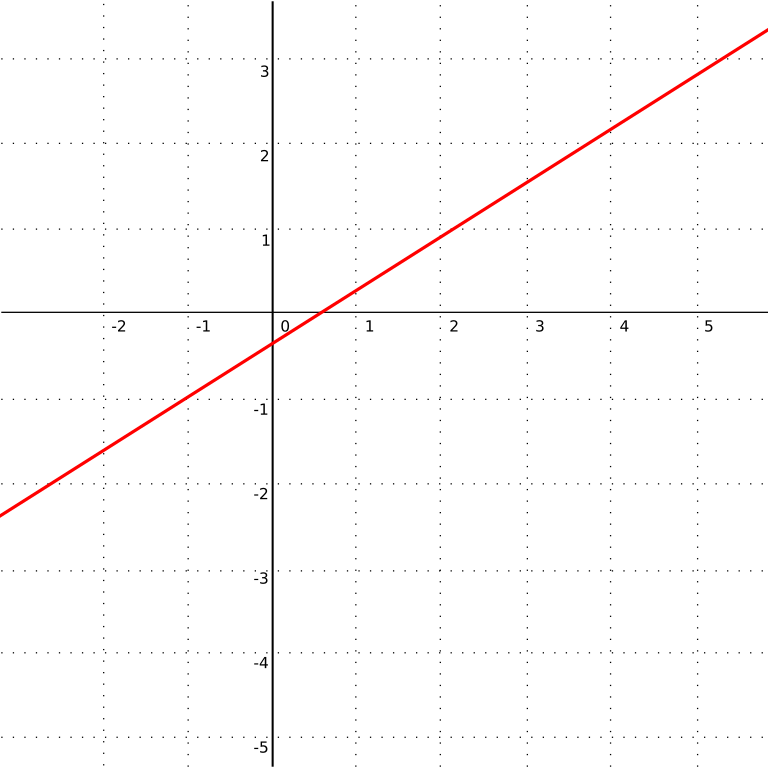
\includegraphics[width=0.3\linewidth]{images/st-line.png}
\end{center}
\end{frame}

\begin{frame}[label={sec:org099c456}]{parametric form}
\begin{columns}
\begin{column}{.5\columnwidth}
For any two vectors \(\mathbf{u},\mathbf{v}\in V\), a
point on the line segment joining them is given
parameterised by \(t\in[0,1]\), as

\begin{align}
  \notag
  \mathbf{p} = f(t) &= (1-t)\mathbf{u} + t\mathbf{v}
\end{align}
\end{column}
\end{columns}
\end{frame}

\begin{frame}[label={sec:orge7ec8cc}]{parametric form}
\begin{columns}
\begin{column}{.5\columnwidth}
Any point on a line in the direction of unit vector
\(\mathbf{u}:\|\mathbf{u}\|_2^2=1\), and an incident
point \(\mathbf{p}_0\) may be given parameterised by
\(t\in\mathbb{R}\) as,

\begin{align}
  \notag
  \mathbf{p} = f(t) &= \mathbf{p}_0 + t\mathbf{u}
\end{align}
\end{column}
\end{columns}
\end{frame}

\begin{frame}[label={sec:orga97ff4f}]{hesse normal form}
\begin{columns}
\begin{column}{.5\columnwidth}
\begin{center}
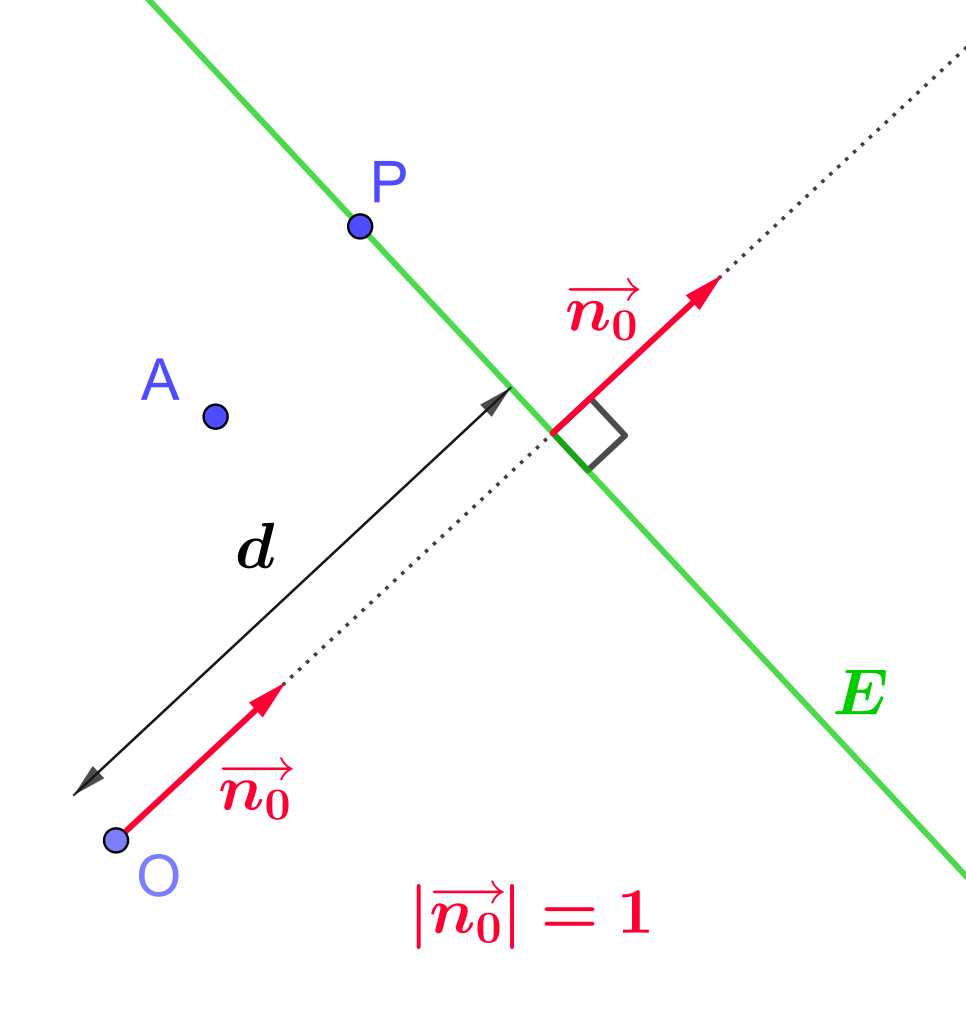
\includegraphics[width=0.7\linewidth]{images/Hesse_normalenform.svg.png}
\end{center}

Distance from the origin \(O\) to the line \(E\) calculated
with the Hesse normal form. Normal vector in red, line
in green, point O shown in blue.
\end{column}

\begin{column}{.6\columnwidth}
Given, \\[0pt]
Normal to the line
\(\mathbf{n}_0:\|\mathbf{n}_0\|_2^2=1\), and \\[0pt]
its distance from origin, \(d\);

\vspace{\baselineskip}
The point on the line is given implicitly as the locus
of all points \(\mathbf{p}\) that satisfy,

\begin{align}
  \notag
  \mathbf{n}_0 \cdot \mathbf{p} - d &= 0
\end{align}
\end{column}
\end{columns}
\end{frame}

\subsection{Conics}
\label{sec:orgaa7a04b}


\begin{frame}[label={sec:org8a945d5}]{circle}
\begin{columns}
\begin{column}{.4\columnwidth}
\begin{figure}[htbp]
\centering
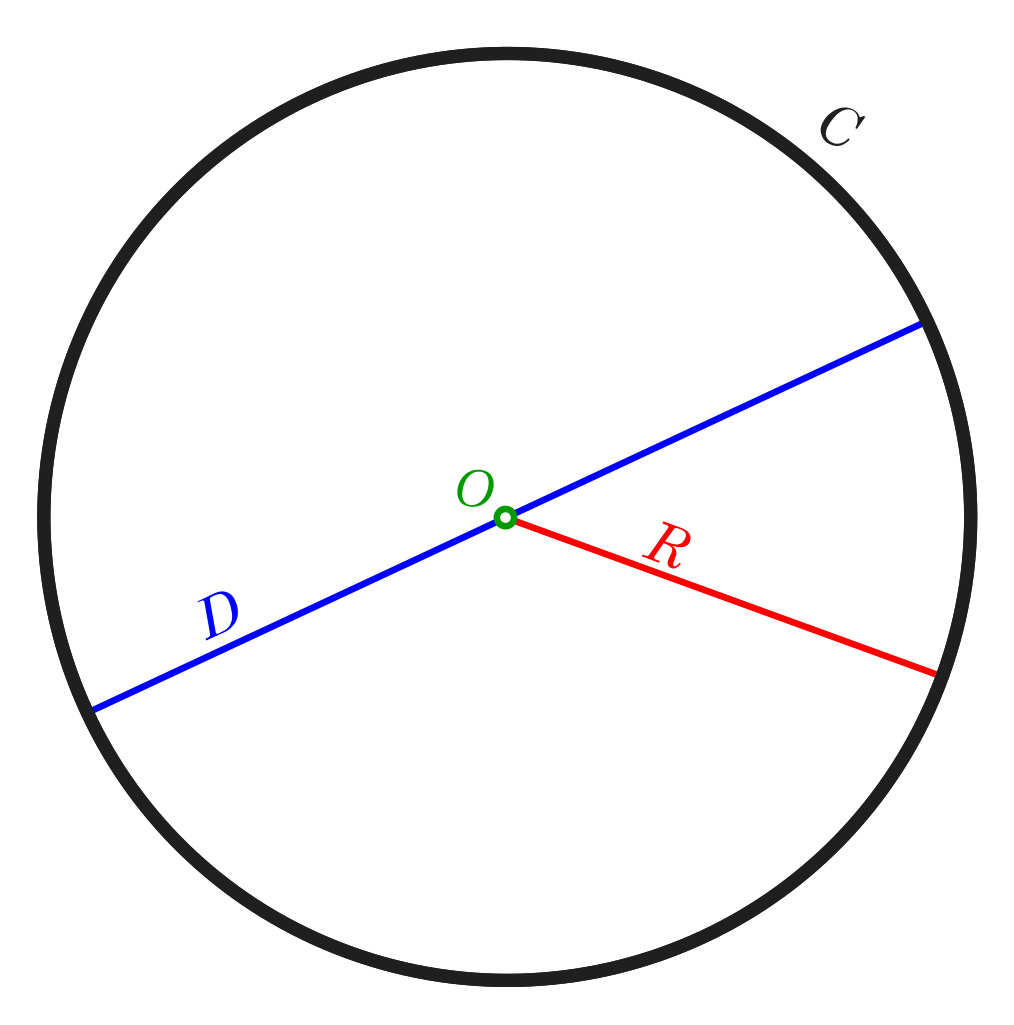
\includegraphics[width=.9\linewidth]{images/Circle-withsegments.svg.png}
\caption{Image Courtesy: \href{https://en.wikipedia.org/wiki/File:Circle-withsegments.svg}{Wikipedia}}
\end{figure}
\end{column}

\begin{column}{.6\columnwidth}
Implicit Form:
\begin{align}
  \notag
  f\left(\begin{matrix}x\\y\end{matrix}\right)
  &= x^2 + y^2 - r^2 = 0
\end{align}

Parametric Form:
\begin{align}
  \notag
  f(r,t)
  &= \begin{bmatrix}r\cos t\\r\sin t\end{bmatrix}
\end{align}
\end{column}
\end{columns}
\end{frame}
\begin{frame}[label={sec:org2d38585}]{ellipse}
\begin{columns}
\begin{column}{.4\columnwidth}
\begin{figure}[htbp]
\centering
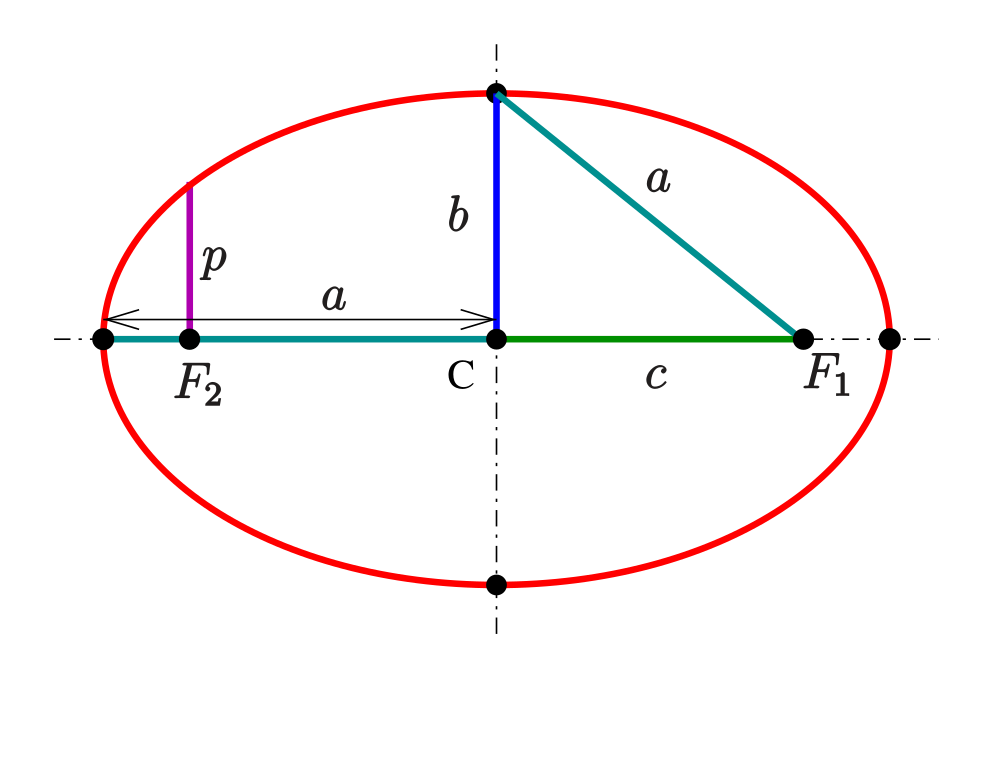
\includegraphics[width=.9\linewidth]{images/Ellipse-param.svg.png}
\caption{Image Courtesy: \href{https://commons.wikimedia.org/wiki/File:Ellipse-param.svg}{Wikipedia}}
\end{figure}
\end{column}

\begin{column}{.6\columnwidth}
Standard form
\begin{align}
  \notag
  f\left( \begin{matrix}x\\y\end{matrix} \right)
  &= \frac{x^2}{a^2} + \frac{y^2}{b^2} - 1 = 0
\end{align}

Parametric Form
\begin{align}
  \notag
  f(t;a,b) &= \begin{bmatrix}
    a\cos t \\ b \sin t
  \end{bmatrix}
\end{align}
\end{column}
\end{columns}
\end{frame}


\section{mid-point algorithm}
\label{sec:org7f99154}

\subsection{Fundamentals}
\label{sec:org8b6be91}

\begin{frame}[label={sec:org1219b3f}]{problem}
In a quantised (pixelated or discrete) 2d plane, find
the set of points that visually approximate a given
curve, say a straight line or a conic.
\end{frame}

\begin{frame}[label={sec:orgb9d85e3}]{method}
\begin{columns}
\begin{column}{.5\columnwidth}
Iteratively, increment along one axes, \\[0pt]
with respect to which, the slope of the curve is
gentle.

{\vspace{\baselineskip}}
Decide whether it is required to increment along the
perpendicular axis or not.

{\vspace{\baselineskip}}
Increment if required.
\end{column}
\end{columns}
\end{frame}

\begin{frame}[label={sec:org6739222}]{example}
\begin{center}
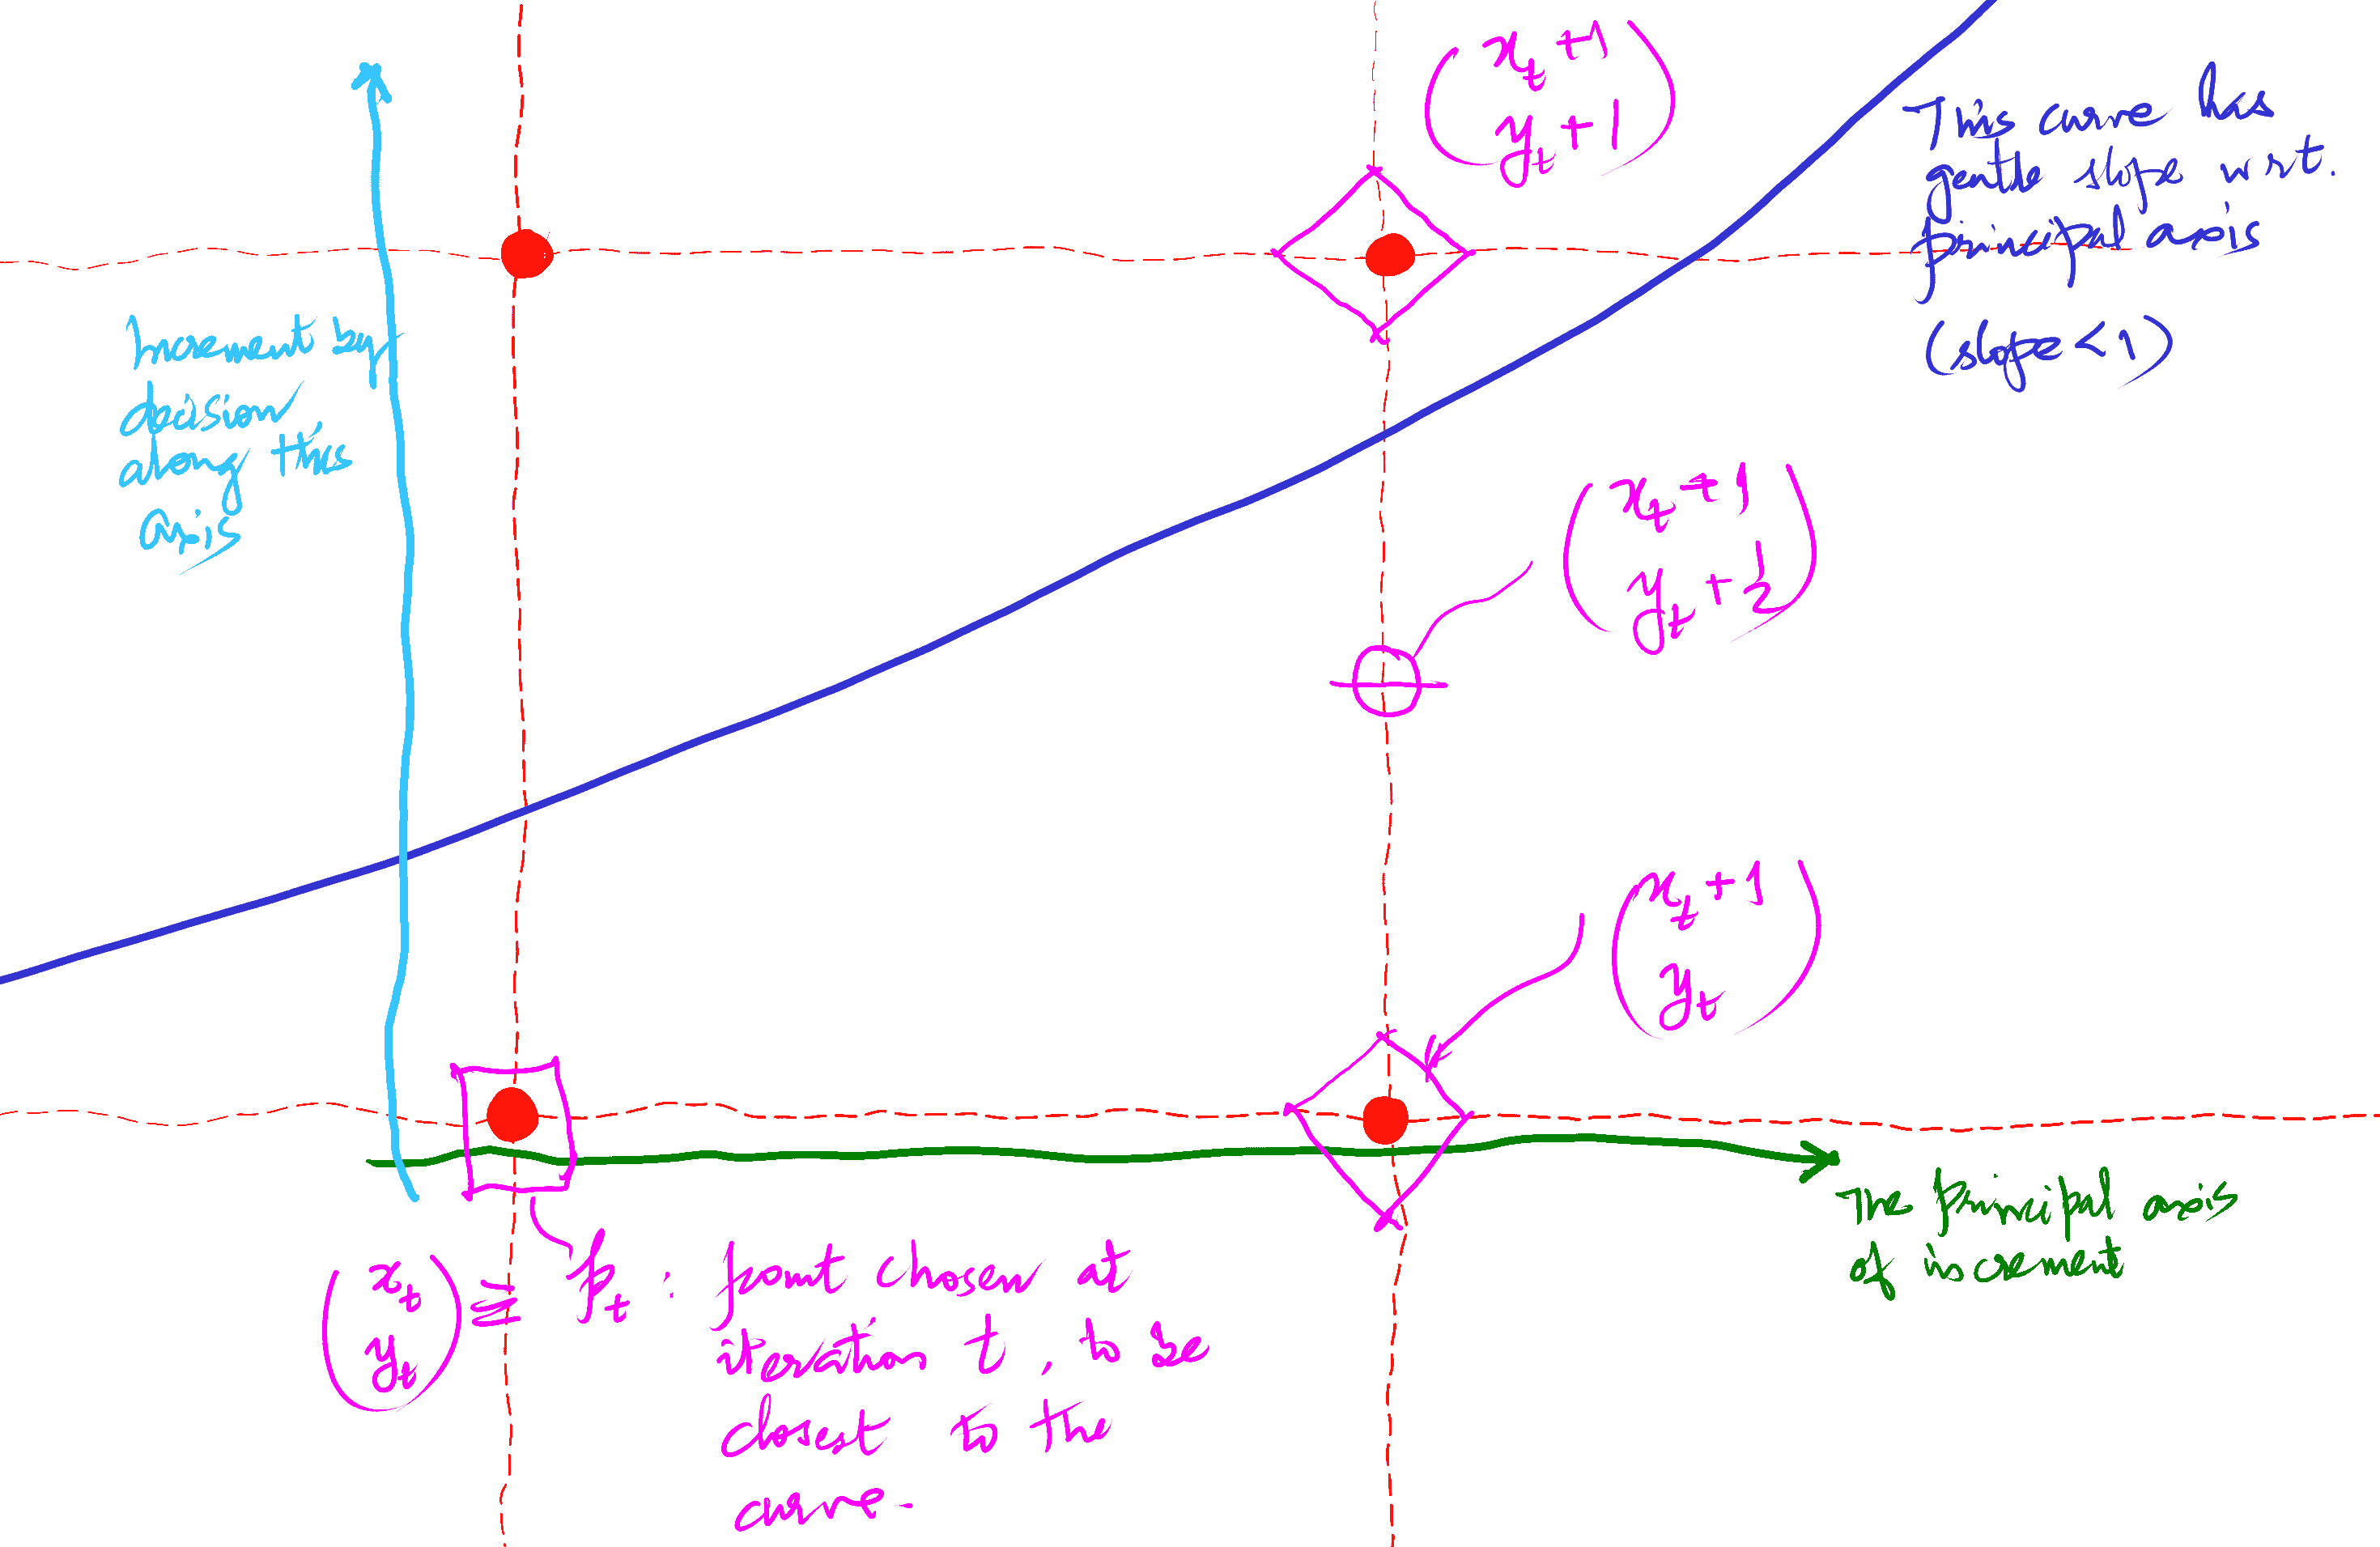
\includegraphics[width=0.8\linewidth]{images/basic-midpoint-algo.png}
\end{center}
\end{frame}

\begin{frame}[label={sec:org27b0457}]{example}
\begin{center}
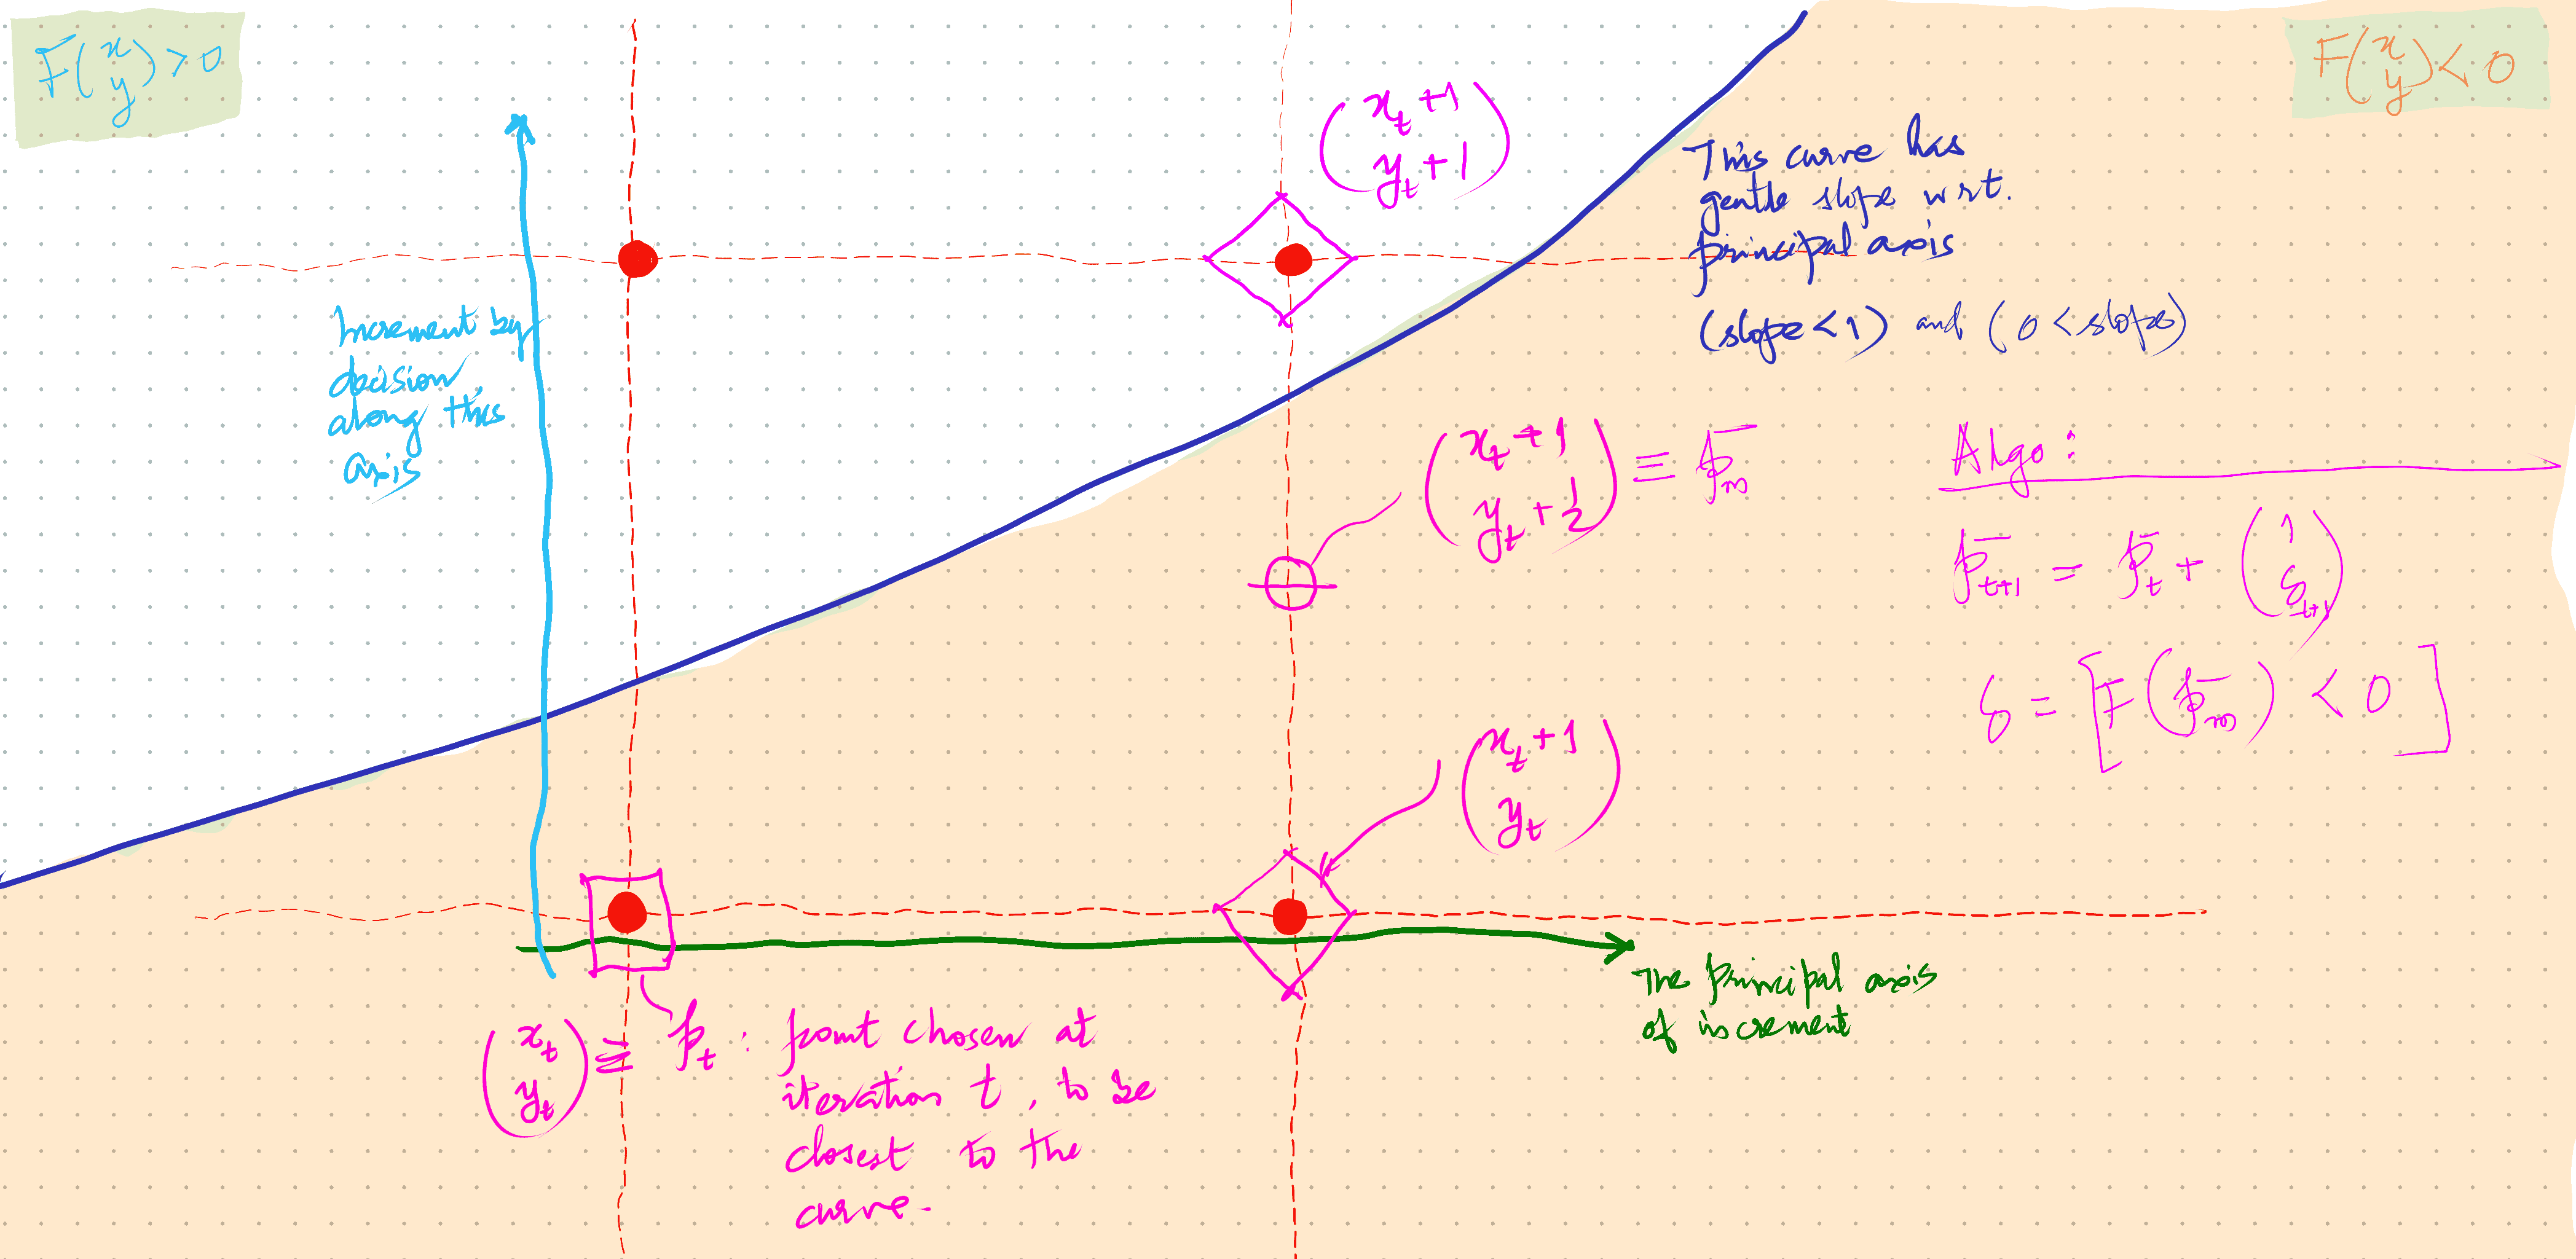
\includegraphics[width=\linewidth]{images/0--mid-point-algo_annotated.png}
\end{center}
\end{frame}

\begin{frame}[label={sec:orgd807adb}]{conditions for application of mid-point algorithm}
\begin{columns}
\begin{column}{.45\columnwidth}
Mid-point algorithm is applicable to a curve within a
given finite interval, \alert{iff}

\begin{enumerate}
\item The curve increases monotonically;
\item The curve increases gradually.
\end{enumerate}


In other words,
\begin{align}
  \notag
  0 &\leqslant \mathrm{d}y \leqslant \mathrm{d}x
\end{align}
\end{column}
\end{columns}
\end{frame}

\begin{frame}[label={sec:org40b3ecc}]{generic algo}
\begin{algorithm}[H]
  \caption{Generic Mid-point Algorithm}
  \DontPrintSemicolon
  \KwIn{$x_0,x_{\mathrm{max}}\in\mathbb{Z}$\hfill\scriptsize
    Start and end x-coordinates.}

  \KwIn{$F:\mathbb{R}^2\to\mathbb{R}$ \hfill
    \scriptsize Signed Distance Function from the curve.}

  \KwOut{$C \equiv
    \{\mathbf{p}_0,\ldots,\mathbf{p}_{\mathrm{max}} \}
    \subset \mathbb{Z}^2$ \hfill \scriptsize Curve in
    discrete 2D space.}

  {$\mathbf{p}_0 \gets \begin{bmatrix} x_0 \\ \lceil
    y_0\rceil \end{bmatrix} \vdash F\left(\begin{matrix}
      x_0 \\ y_0 \end{matrix}\right) = 0$}


\For{$t\in\{1,\ldots,\mathrm{max}\}$}{
  $\mathbf{p}_{\mathrm{mid}}\gets\mathbf{p}_{t-1}+\begin{pmatrix}1\\
    \frac12\end{pmatrix}$

  $\delta_t\gets I[F(\mathbf{p}_{\mathrm{mid}})<0]$

  $\mathbf{p}_{t}\gets\mathbf{p}_{t-1}+\begin{pmatrix}
    1 \\ \delta_{t} \end{pmatrix}$
  }
\end{algorithm}
\end{frame}


\subsection{Straight Line}
\label{sec:orgc8fc694}

\begin{frame}[label={sec:org997e59d}]{characterising straight lines}
\begin{align*}
  F(x,y)
  &= Ax-By+C \\
  0 \leqslant \mathrm{d}y / \mathrm{d}x \leqslant 1 \quad
  &\mapsto \quad 0 \leqslant A \leqslant B
  &&\textsc{\ldots case 1} \\
  -1 \leqslant \mathrm{d}y / \mathrm{d}x \leqslant 0 \quad
  &\mapsto \quad 0 \leqslant A \leqslant -B
  &&\textsc{\ldots case 2} \\
  0 \leqslant \mathrm{d}x / \mathrm{d}y \leqslant 1 \quad
  &\mapsto \quad 0 \leqslant B \leqslant A
  &&\textsc{\ldots case 3} \\
  -1 \leqslant \mathrm{d}x / \mathrm{d}y \leqslant 0 \quad
  &\mapsto \quad 0 \leqslant -B \leqslant A
  &&\textsc{\ldots case 4}
\end{align*}
\end{frame}

\begin{frame}[label={sec:org335478d}]{mid-point algo for st. line}
\begin{algorithm}[H]
  \caption{Mid-Point Algorithm for Straight Line (intermediate attempt)}
  \DontPrintSemicolon
  \KwIn{$x_0,x_{\mathrm{max}}\in\mathbb{Z}$\hfill\scriptsize
    Start and end x-coordinates.}

  \KwIn{$a,b,c\in\mathbb{Z} \vdash 0\leqslant a < b;
    b\;\mathrm{even}$ \hfill \scriptsize Coefficients:
    $F(x,y)=ax-by+c$. \textbf{Rem:} \alert{$-by$}.}

  \KwOut{$C \equiv
    \{(x_0,y_0),\ldots,(x_{\mathrm{max}},y_{\mathrm{max}})
    \} \subset \mathbb{Z}^2$ \\\scriptsize An ordered
    sequence; a curve in discrete 2D space.}

  $y_0\gets\lceil\frac{ax_0+c}{b}\rceil$
  
  $\delta_0\gets ax_0-by_0- \frac b2 +c$
  \hfill{\scriptsize \textbf{Rem:}
    \alert{$-by_0 - \frac b2$}; $\frac b2\in\mathbb{Z}$
    because $b$ even.}

  \For{$t\in\{1,\ldots,\mathrm{max}\}$}{
    $x_t\gets x_{t-1} + 1$

    $\delta_t\gets \delta_{t-1} + a -
    b\cdot I[\delta_{t-1}<0]$

    $y_t \gets y_{t-1} + I[\delta_t<0]$
  }
\end{algorithm}
\end{frame}

\begin{frame}[label={sec:org432c274}]{mid-point algo for st. line}
\begin{algorithm}[H]
  \caption{Mid-Point Algorithm for Straight Line}
  \DontPrintSemicolon
  \KwIn{$x_0,x_{\mathrm{max}}\in\mathbb{Z}$\hfill\scriptsize
    Start and end x-coordinates.}

  \KwIn{$a,b,c\in\mathbb{Z} \vdash 0\leqslant a < b;
    b\;\mathrm{even}$ \hfill \scriptsize Coefficients:
    $F(x,y)=ax-by+c$. \textbf{Rem:} \alert{$-by$}.}

  \KwOut{$C \equiv
    \{(x_0,y_0),\ldots,(x_{\mathrm{max}},y_{\mathrm{max}})
    \} \subset \mathbb{Z}^2$ \\\scriptsize An ordered
    sequence; a curve in discrete 2D space.}

  \textbf{Init:} $C$ as a new Array.

  \textbf{Init:} $x,y,\delta$ as integers.

  $x\gets x_0$

  $y\gets\lceil\frac{ax+c}{b}\rceil$
  
  $\delta\gets ax-by- \frac b2 +c$
  \hfill{\scriptsize \textbf{Rem:}
    \alert{$-by - \frac b2$}; $\frac b2\in\mathbb{Z}$
    because $b$ even.}

  $C\cdot$ Push($(x,y)$)

  \For{$t\in\{1,\ldots,\mathrm{max}\}$}{
    $x\gets x + 1$

    $\delta\gets \delta + a -
    b\cdot I[\delta<0]$

    $y \gets y + I[\delta<0]$

    $C\cdot$ Push($(x,y)$)
  }
\end{algorithm}
\end{frame}

\begin{frame}[label={sec:org415da02}]{}
\end{frame}
\subsection{Circle}
\label{sec:orgc5aee12}

\againframe{sec:org40b3ecc}

\begin{frame}[label={sec:org62c78f6}]{}
\end{frame}
\end{document}
